% siminos/blog/baroclinic.tex
% $Author$ $Date$

\chapter{Baroclinic flows}
\label{chap:baroclinic}

\section{Setup}
\label{s:review}

    \PC{the text here is taken from the pipes/slice article,
        needs to be rewritten}
The flow to be considered is that of $N$ layers of $2D$
incompressible viscous fluid
confined within a rectangular channel, driven by a mean
unit velocity added to the top layer
in the stream-wised direction.  The Reynolds number is defined as
$\Reynolds = ?U L / \nu?$, where $U$ is the mean velocity??? of the flow,
$L$ is the channel span-wise width, and $\nu$ is the kinematic viscosity. We
scale lengths by $L/2$ and velocities by $2U$ in the \NSe\ for
$\vec{u}$, the deviation from the laminar flow
\eqv\ $U(r)=1-r^2$,
    \PC{write baroclinic equations here}
\beq
\frac{\partial\vec{u}}{\partial t} + U(r)\cdot\bnabla\vec{u} +
\vec{u}\cdot\bnabla U(r) + \vec{u}\cdot\bnabla\vec{u} = - {\bnabla} p
+ \frac{4\beta}{\Reynolds}\hat{{\bf z}} +
\frac{1}{\Reynolds}{\bnabla}^2 \vec{u}\,, \quad \nabla \cdot \vec{u} =
0 \,.
\ee{NavStokesDev}
Here the dimensionless variable $\beta$ is the fractional pressure
gradient, additional to the laminar flow, required to maintain a
constant mean velocity $U$. A Reynolds number $\Reynolds_p$, based on
the applied pressure gradient, is given by $\Reynolds_p = ??$,
whereas the friction Reynolds number is
$\Reynolds_{\zeit}=??$. The \NSe\ are formulated in
cylindrical-\-polar coordinates, where $(x, y, n)$ are the
stream-wise, span-wise positions and layer,
respectively. The full fluid velocity field $U(r)\hat{{\bf z}} +
\vec{u}$ is represented by $[u,v,w,p](r,\theta,z)$, with $u$, $v$ and
$w$ respectively the radial, azimuthal and stream-wise velocity
components, and $p$ the pressure. In numerical simulations no-slip
boundary conditions are imposed at the side walls and
periodic boundary conditions in the stream-wise $x$
direction. The computational domain is
\[
\bCell={(x,y,n) \in
  [0,2\pi/\alpha]\times[0,2]\times[n]}
\,,
\] where
$L=2\pi/\alpha$ is the length of the domain.

This study is conducted at $\Reynolds = ??$, with $N=2$ and
$\alpha=1.25$, corresponding to a short $L\simeq 4\times 2$-periodic
cell in
the stream-wise direction,
\begin{align}
\bCell~ &= [1,\pi,2\pi/1.25] &\approx [90, 283, 452] \;\;\;
\text{wall units}
    \label{shortPipe}
\end{align}
At
$\Reynolds = ??$ this computational cell empirically sustains
turbulence for very long times. In average the additional pressure
fraction required to support turbulence while keeping constant mass-flux
is $\langle\beta\rangle_t=0.70$, yielding friction Reynolds number
$\Reynolds_{\zeit}=90.3$.  At this Reynolds number and geometry one domain
width $2$ corresponds to about $90?$ wall units. The domain size
\eqref{shortPipe} was chosen as a compromise between the computational
preference for small domains {\em vs.} the need for the domain to be
sufficiently long to accommodate turbulent dynamics. In addition,
restricting the largest wavelength is very useful in identifying key
coherent structures characterizing turbulent dynamics\rf{HaKiWa95}.
Although the cells studied in this paper are short, the two-dimensional
states explored here  by \eqva\ and their unstable manifolds are
strikingly similar to typical states in longer domains.

% \subsection{Numerical discretization}
% \label{s:NumDiscr}

A choice of a basis set for function space of solutions is greatly aided
by the symmetries of the flow. Baroclinic domains are stream-wise (in
numerical work) periodic, so deviation velocity field $\vec{u}$ and
deviation pressure in the \NS\ equations \refeq{NavStokesDev} are
expanded in Fourier modes in the stream-wise and span-wise directions,
\beq
\vec{u}(x,y,n) = \sum_{|k|<K} \sum_{|m|<M} \vec{u}_{nkm}
\, \mathrm{e}^{\mathrm{i}(\alpha x z+ m y)}
\,,
\ee{pipeDiscr}
whereas the finite-difference method is used in the radial direction.
Flow states are typically characterized by the instantaneous kinetic
energy of their deviation from laminar flow, $E = \frac{1}{2}
\Norm{\vec{u}}^2$, and energy dissipation rate $D =
1/\Reynolds\Norm{\bnabla \times \vec{u}}^2$. The dissipation rate is
balanced by the energy fed into the flow as
\beq
\dot{E}=I-D
\,,
\ee{Power=I-D}
where
\(
I =\oint dS \, ({\bf n}\cdot\vec{u})\, p
\)
is the additional instantaneous external power required to maintain
constant flux, over that of the laminar flow.  For \reqva\ the kinetic
energy is constant and so $D=I$, such solutions sit on the diagonal in
\reffig{f:energyBalance}, whereas for relative periodic orbits the kinetic
energy is time-periodic, with $\timeAver{D}=\timeAver{I}$ only for
long-time averages.
    \PC{
    It would be instructive to supplement $(I,E)$,
    % \reffig{fig:M1Orb},  \reffig{heterodissRPO}
    by the $(I,D)$  plot as well
    }

\begin{figure}
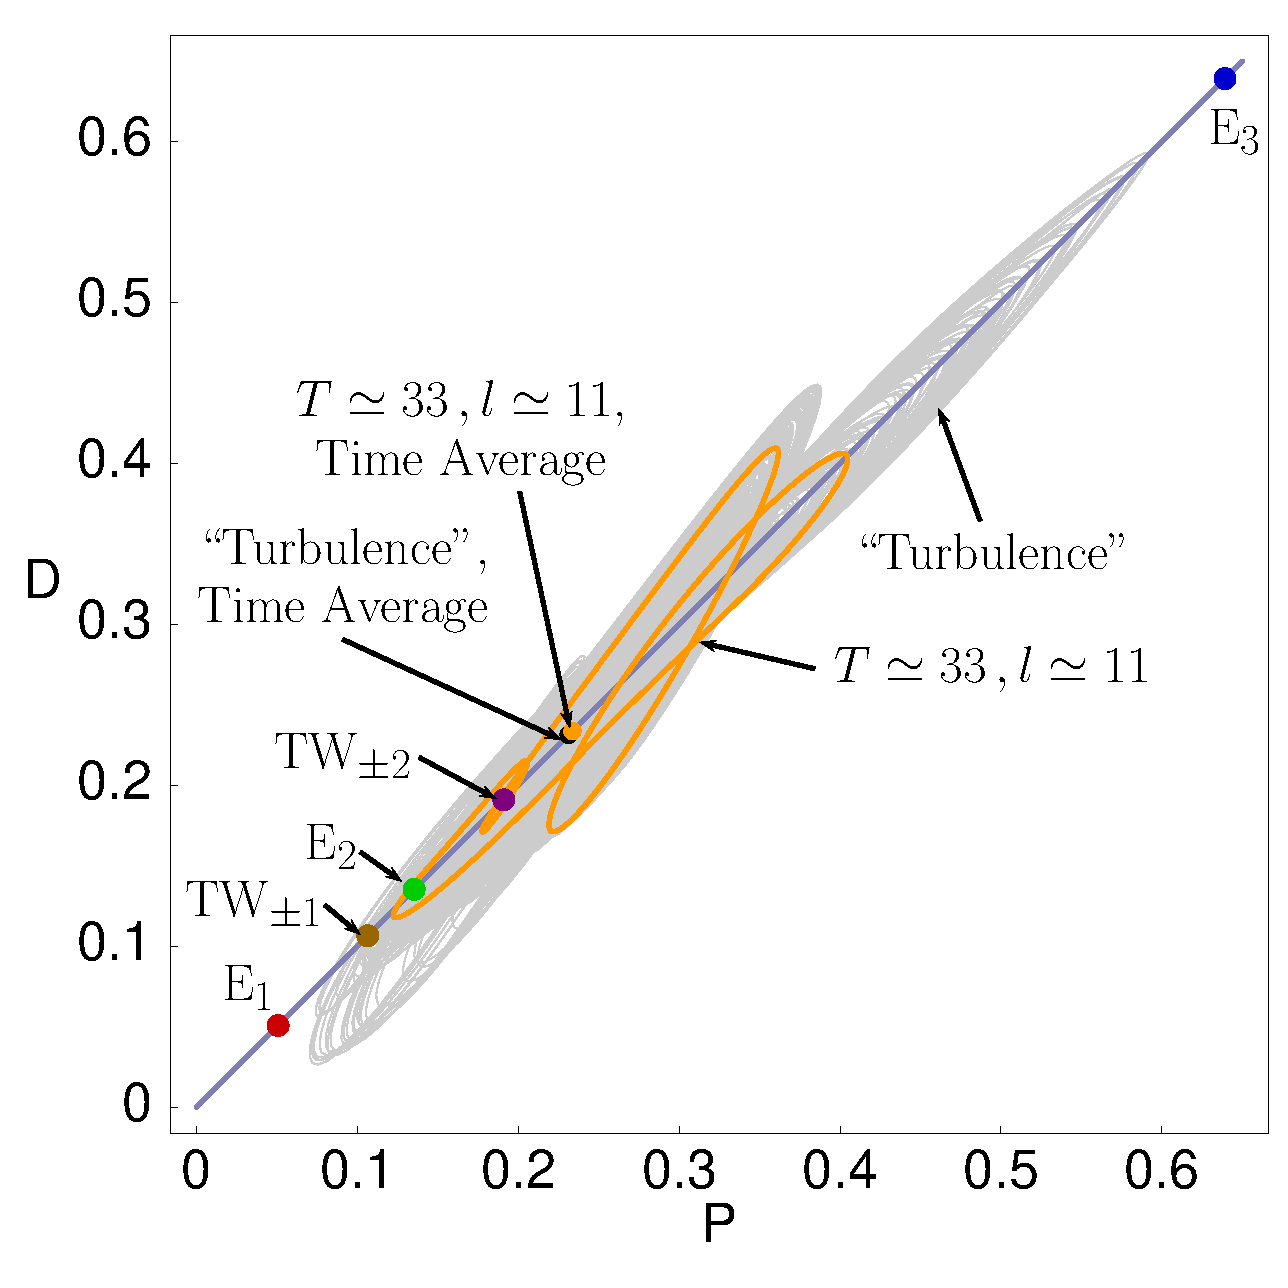
\includegraphics[width=0.45\textwidth]{energyBalance_pst}
\caption{
    (Color online) Normalised $(I,D)$ projection \refeq{Power=I-D}
of the \rpo s  [Bum]
    (red) and [Bam]  (blue). Also shown are all \reqv\ Mothers and Nigels
    used as \template s in this paper.
    Rate of energy input at the walls $I$ versus dissipation $D$.
    }
\label{f:energyBalance}
\end{figure}


\subsection{{\StateDsp} visualization of fluid flows}
\label{s:visualStatSp}

Hopf\rf{hopf48} envisioned the function space of {\NS} velocity fields as
an infinite-dimensional \statesp\ $\pS$ in which each instantaneous state
of $3D$ fluid velocity field $\bu(\bx)$ is represented as a unique point
$\ssp$. In our particular application we can represent $\ssp =
(\vec{u}_{nkm})$ as a vector whose elements are the primitive
discretization variables \refeq{pipeDiscr}, but, as we shell show below,
other coordinatizations are more powerful. The distance between two
points in \statesp\ is here measured as
\beq
  \Norm{\ssp-\ssp'}^2  = \braket{\ssp-\ssp'}{\ssp-\ssp'} =
%\frac{1}{V}
\int_\bCell \! d \bx \;
(\vec{u}-\vec{u}') \cdot (\vec{u}-\vec{u}')
\,.
\ee{innerproduct}
Whether one uses this {`energy norm'} or another norm, depends very much
on the application. In the study of `optimal perturbations' that move a
laminar solution to a turbulent one, both energy\rf{TeHaHe10} and
dissipation\rf{LoCaCoPeGo11} norms have been used.  In our searches
for \reqva\ and \rpo s (see \refsect{s:rpos}) we find it advantageous to
use a `compensatory' norm % \refeq{compensNorm}.
\beq
   \Norm{\vec{u}}_c^2 \,=\, \braket{\vec{u}}{\vec{u}}_c
   \,=\, \frac{1}{2}\,\int_V (9\,u \cdot u + 9\,v \cdot v + w \cdot w)
        \, \mathrm{d}V
\,,
\ee{compensNorm}

The $N$-layer $2D$ velocity field $\vec{u}_{knm}(\zeit)$ obtained by
integrating the \NS\ equations in time can hence be seen as trajectory
$\ssp(\zeit)$ in $\approx ?100,000$ dimensional space spanned by the free
variables of our numerical discretization, with the \NS\ equations
\refeq{NavStokesDev} rewritten as
\beq
   \dot{\ssp} = \vel(\ssp) ,
   \qquad
   \ssp(\zeit) = \ssp(0)
            + \int_0^\zeit \! \mathrm{d}\zeit' \, \vel(\ssp(\zeit'))
\,,
\ee{symbolicNS}
where the current state of the fluid $ \ssp(\zeit)$ is the time-$\zeit$
forward map of the initial fluid state  $\ssp(0)$. Visualizations
of this trajectory are of necessity projections onto two or three
dimensions. It is customary in the literature to monitor the flow in
terms of the symmetry-invariant physical energy, dissipation and power
input observables $(E(\zeit),D(\zeit),I(\zeit))$,
as in \reffig{f:energyBalance}, but such plots may obscure
some of the most relevant features of the flow. Other common
visualization are discretization-method dependent projections onto
two or three Fourier components of the flow, but with choices of modes both
arbitrary and unphysical, as in a highly nonlinear flows many Fourier
modes are strongly coupled and of comparable magnitude.

Recently, Gibson \etal\rf{GHCW07} have shown that the dynamics of
different regions of {\statesp} can be elucidated by projections onto
physically motivated orthonormal basis sets $\{\be_1, \be_2, \cdots,
\be_n\}$ that span sets of important fluid states $\bu_A$, $\bu_B$,
$\dots$, such as {\eqv} states and their eigenvectors. Such
visualizations are a prerequisite to uncovering the interrelations
between (the infinite number of) invariant solutions, and constructing
symbolic dynamics partitions of \statesp\ needed for a systematic
exploration of turbulent dynamics. The evolving fluid state $\bu(\zeit)$
is then projected onto this basis using the
% $L^2$
inner product \refeq{innerproduct},
\beq
\ssp(\zeit) =(\ssp_1, \ssp_2, \cdots, \ssp_n, \cdots)(\zeit)
    \,,\qquad
\ssp_n(\zeit) = \braket{\bu(\zeit)}{\be_n}
\,.
\ee{intrSspTraj}
This low-dimensional projection can be viewed in any of the $2D$ planes
$(\ssp_m, \ssp_n)$ or in $3D$ perspective views $(\ssp_{\ell},\ssp_m,
\ssp_n)$, see \reffig{f:MeanVelocityFrame}. The {\stateDsp} portraits are
{dynamically intrinsic}, since the projections are defined in terms of
intrinsic solutions of the equations of motion, and {representation
independent}, as the inner product \refeq{innerproduct} is independent of
the numerical discretization. It is worth emphasizing that the method
affords low-dimensional {\em visualization} without any low-dimensional
{\em modeling} or dimension reduction; the dynamics are computed with
fully-resolved direct numerical simulations. Although the use of
particular \reqva\ to define low-dimensional projections may appear
arbitrary, such a choice turns out to be very useful when the turbulent
flow is chaperoned by a few invariant solutions and their unstable
manifolds, as has been shown in other low Reynolds number
settings\rf{GHCW07}.



\section{Daily blog, point by point}
\label{sect:blogBaroclin}


\begin{description}

\item[2011-05-27 Predrag, weather report from Snowbird DS11]
	\toCB
Learned from Pierrehumbert that the baroclinic models are to weathermen
what ``harmonic oscillator'' is to quantum mechanics. It has a continuous
East-West translational symmetry, \ie, in a periodic box it needs to be
sliced (the \SOn{2} of periodic box quotiented out).

Tried to proselytize Christian Wolfe\rf{WoSa07}, Scripts,  make him slice
the baroclinic instability, and, perchance, if I get him there, recycle
it, former Gibson style. Pierrehumbert says that this would be persuasive
to weather people, convince them to go looking for exact unstable
invariant solutions. After one hour Wolfe said he was converted.

Tried ditto with Pierrehumbert and Silber postdoc Yi-Ping Ma (Knobloch
trained, has worked with Spiegel at Woods Hole GFD). He does not know any
geophysical fluid dynamics yet, so I'm sceptical that he will do anything.

\item[2011-05-27 Annalisa Bracco]
If you ever need a code that produce baroclinic instability, I have
plenty. Worked with the Baroclinic Instability Man as a postdoc. I also
have an easy atmospheric model (global, on a sphere etc) that reproduces
very well baroclinic instability as per observations and can be run as
aqua-planet to simplify things.

\item[2011-05-27 Predrag]
Joe Pedlosky? We plumbers could make Joe happy? Let's do it before
August, in time for Woods Hole. The first step is to slice your
simulations for a minimal periodic cell of interest (narrow but
turbulent). The second step might be either to determine ``physical
dimension'' using Wolfe-Samelson\rf{WoSa07} Lyapunov vectors (that is
just simulation) or find some traveling waves (that is Krylov-Arnoldi
nontrivial work, but for low-dimensional discretizations might be doable
by Newton).

\item[2011-10-15 Annalisa]
'Baroclinic' means that the instability is driven by density difference;
'barotropic' means not. Annalisa has shown Predrag some simulations.
Baroclinic instability is modeled by a 2-layer incompressible viscous
fluid in a channel with no-slip side walls, periodic in streamwise
direction, top layer driven by `atmospheric stream', \ie\ a constant
total streamwise volume flow per unit time. She simply imposes uniform
streamwise velocity of unit size, ignoring the boundary condition (could
use a parabolic profile). With free slip the layers are still unstable in
the same way, just the boundary behavior is different. Oceanographers
prefer no-slip, perhaps because of coastal stream. The bottom layer is
not forced, no slip, no Eckman layer (Eckman layer models friction at the
bottom; that would make sense when she works with 50 layers, but not
two). The two layers are coupled by the difference $\Phi_2 - \Phi_1$.
Laplacian of stream function is vorticity. Each layer is computed in
terms of vorticity equations as a 2-dimensional fluid. The lower layer
has higher fluid density, and they are coupled across their interface by
difference of vorticity. This is about factor two; it is related to the
R\"osby deformation radius $L_R$. The spanwise $y$ width is $L_R/2\pi =
1/2$. Unless the width is larger than $L_R$, no instability. The
stream-wise aspect ration is about 8.

They tend to the barotropic solution (vortices rotating the same way on
top and bottom).

%%%%%%%%%%%%%%%%%%%%%%%%%%%%%%%%%%%%%%%%%%%%%%%%%%%%%%%%%%%%%%%%%%%%%
\FIG{
 (a)\includegraphics[width=0.95\textwidth]{111018t32_NL}
\\
(b)\includegraphics[width=0.95\textwidth]{111018reduced}
 }{}{
2 layers: top, bottom.
(a)
The usual domain $L=8$.
(b)
The reduced domain $L=4$, initial conditions starting
from a linear solution. The energy is not yet fully equilibrated.
The longer
cell (a) behaves pretty much the same way, but overall
the circulation is a bit stronger.
}{2layerBclin}
%%%%%%%%%%%%%%%%%%%%%%%%%%%%%%%%%%%%%%%%%%%%%%%%%%%%%%%%%%%%%%%%%%%%%


Discussion of solutions:
\begin{enumerate}
  \item [1)]
is linear: dropped the nonlinear term \ie\ the Jacobian of the vorticity
and the stream function. Instability is seeded by a small random field of
prescribed power spectrum, but the resulting instability is a localized
wave (about 3 rolls) with streamwise/spanwise ratio of about 1/2 set
$L_R$. That sets the scale of the instability off the laminar solution.
Initial noise does not matter, as the instability grows very fast. The
two layer vorticities are opposite.

  \item [2)] is fully nonlinear, all other parameters the same.

  \item [3)]
\end{enumerate}

\item[2011-10-18 Annalisa]

\refFig{2layerBclin}\,(a)
The usual domain $L=8$, 2 layers. Note that as
for initial conditions, the overall the flow is more energetic.

\refFig{2layerBclin}\,(b)
The reduced domain $L=4$, 2 layers. Correct initial conditions, starting
from a linear solution. The energy is not yet fully equilibrated. One
problem I can see is that the periodic boundary conditions may prevent
perfect equilibration. Anyway, it'll be running over night. The longer
cell \refFig{111018t32_NL} behaves pretty much the same way, but overall
the circulation is a bit stronger.

\item[2011-10-19 Annalisa]
There is a barotropization issue, likely due to the periodic boundaries.
My guess is that we'll not need a very long simulation and we can live
with a non perfectly stationary state (essentially the eddies that form
in the equilibrated solution prefer to be barotropic -same sign top and
bottom layer- because they are more stable and in the absence of
viscosity, \etc\ they are an exact solution of \NS), and the simulation goes
into a state that resembles the long-term state for 2-d turbulence. If we
could work only over times $\sim $40-70 we should be all set.

For now the time
is just in code units, I'll convert it in something meaningful once we
decide on which run to use, \etc.

\item[2011-10-20 Predrag]
Bit worried if we are in transient turbulence, on the way to a
barotropic state, but might work out... (will include 111018time50,
111018time70 and 111018time100 later...)


\end{description}
